    %https://gateoverflow.in/333196/gate-cse-2020-question-35?show=333279

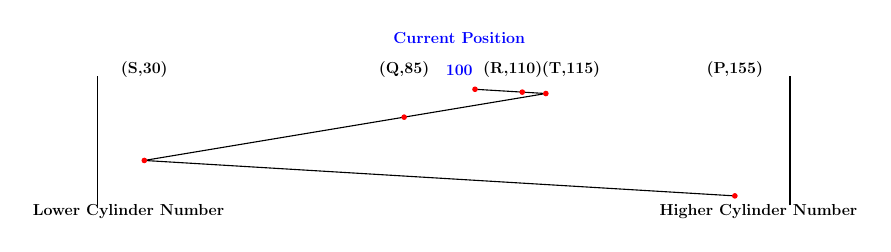
\begin{tikzpicture}[scale = 0.4,font = \bfseries, transform shape]
\Large
\draw (-12,-2.3) -- (-12,1.8);
\draw (10,-2.3) -- (10,1.8);
\draw (0,1.385) -- (1.5,1.295);
\draw (1.5,1.295) -- (2.25,1.25);
\draw (2.25,1.25) -- (-2.25,0.5);
\draw (-2.25,0.5) -- (-10.5,-0.875);
\draw (-10.5,-0.875) -- (8.25,-2);

\filldraw [red] (0,1.385) circle (2pt);
\filldraw [red] (1.5,1.295) circle (2pt);
\filldraw [red] (2.25,1.25) circle (2pt);
\filldraw [red] (-2.25,0.5) circle (2pt);
\filldraw [red] (-10.5,-0.875) circle (2pt);
\filldraw [red] (8.25,-2) circle (2pt);

\node at (-11,-2.5) {Lower Cylinder Number};
\node at (9,-2.5) {Higher Cylinder Number};
\node at (-10.5,2) {(S,30)};
\node at (-2.25,2) {(Q,85)};
\node at (1.20,2) {(R,110)};
\node at (3.05,2) {(T,115)};
\node at (8.25,2) {(P,155)};
\node[text=blue] at (-0.5,3) {Current Position};
\node[text=blue] at (-0.5,2) {100};

\end{tikzpicture}